\documentclass[unicode]{beamer}
\usepackage[T2A]{fontenc}
\usepackage[utf8]{inputenc}
\usepackage[russian]{babel}
\usepackage{cmap}
\usepackage{amssymb,amsfonts,amsmath,mathtext}
\usepackage{graphicx}
% XeTeX packages
\usepackage[cm-default]{fontspec} % or install lmodern and remove cm-default opt
\usepackage{xunicode} % some extra unicode support
\usepackage{xltxtra} % \XeLaTeX macro
\defaultfontfeatures{Scale=MatchLowercase,Mapping=tex-text}

\setromanfont{Charis SIL}
\setsansfont{Charis SIL}
\setmonofont{Charis SIL}

\usepackage{geometry}
\geometry{left=0mm}
\geometry{right=0mm}
\geometry{top=0cm}
\geometry{bottom=0cm}

\usepackage{array}

\setbeamerfont{institute}{size=\normalsize}
\graphicspath{{images/}}
\usetheme{CambridgeUS}
\useoutertheme{shadow}
\useinnertheme{rounded}
\usecolortheme{beaver}
\usefonttheme{professionalfonts}


\title[Расширение функционала системы управления проектами Redmine]{
Разработка расширений для системы управления проектами Redmine
}
\author[Кандауров О.\,В.]{Студент 5-го курса О. Кандауров}
\institute{
Научный руководитель: ст. преподаватель Парамонов~И.\,В.
}
\date{}
\begin{document}
\maketitle

\begin{frame}
\transwipe[direction=90]
\frametitle{Системы управления проектами}
\begin{columns}
\begin{column}{0.45\textwidth}
\begin{itemize}
  \item Оценка и разработка
  \item Планирование
  \item Постановка задач
  \item Управление бюджетом
  \item Распределение ресурсов
  \item Взаимодействие
  \item Документирование
\end{itemize}
\end{column}
\begin{column}{0.55\textwidth}
\centerline{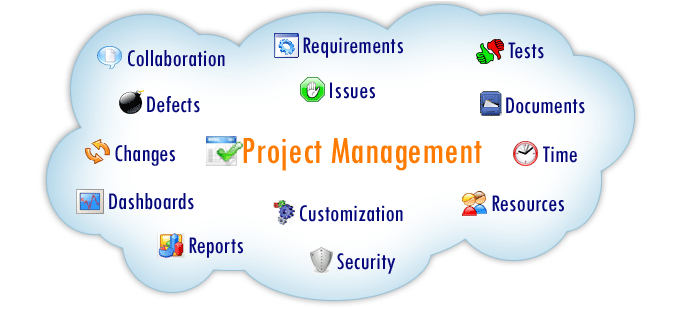
\includegraphics[width=1\textwidth]{project-management-software.png}}
\end{column}
\end{columns}
\end{frame}

\begin{frame}
\transwipe[direction=90]
\frametitle{Идеальная система}
\begin{tabular}{ >{\centering\arraybackslash}m{0.4\textwidth}  >{\centering\arraybackslash}m{0.6\textwidth} }
\begin{minipage}{5cm}
\begin{block}{}
\fontsize{10pt}{12pt}
\begin{itemize}
  \item Требования изменяются
  \item Приходят новые технологии
  \item Ошибки
  \item Стремление к совершенству
\end{itemize}
\end{block}
\end{minipage}&
\begin{minipage}{6cm}
\begin{block}{}
\fontsize{10pt}{12pt}
\begin{itemize}
  \item Усовершенствование функционала
  \item Добавление нового функционала
  \item Исправление дефектов
  \item Кастомизация
\end{itemize}
\end{block}
\end{minipage}\\
\end{tabular}
\hspace{1cm}
\centerline{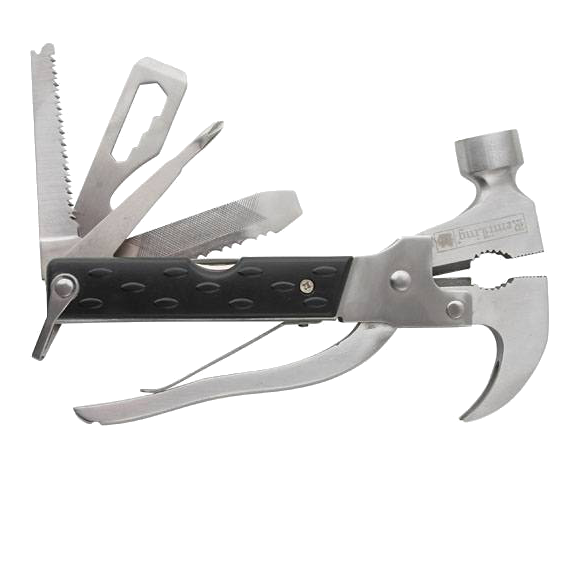
\includegraphics[width=6cm]{super-hammer.png}}
\end{frame}

\begin{frame}
\transwipe[direction=90]
\frametitle{Постановка задачи}
\begin{block}{}
\begin{itemize}
  \item Выбрать систему управления проектами
  \item Изучить возможности расширения / внесения изменений
  \item Добавить необходимый функционал  / Исправить дефекты
  \item Организовать хранение нарабаток
\end{itemize}
\end{block}
\end{frame}

\begin{frame}
\transwipe[direction=90]
\frametitle{Redmine}
\begin{columns}
\begin{column}{0.6\textwidth}
\begin{itemize}
  \item Работает в браузере
  \item Открытые исходные коды
  \item Богатая функциональность
  \item Интеграция с репозиториями
  \item Расширяемость (300+ плагинов)
  \item Активно развивается
\end{itemize}
\end{column}
\begin{column}{0.4\textwidth}
\centerline{
\includegraphics[width=1\textwidth]{redmine-logo.pdf}}
\end{column}
\end{columns}
\end{frame}

\begin{frame}
\transwipe[direction=90]
\frametitle{Способы внесения изменений}
\begin{tabular}{ >{\centering\arraybackslash}m{3.5cm}  >{\centering\arraybackslash}m{5cm} }

\includegraphics[width=1.5cm]{Ruby_on_Rails.pdf}&
\begin{minipage}{3in}
\begin{block}{Система плагинов Redmine (Rails engines)}
\begin{itemize}
  \item Redmine view/model hooks
  \item Controller filters
  \item ActiveRecord callbacks
\end{itemize}
\end{block}
\end{minipage}\\


\includegraphics[width=1.5cm]{Ruby_logo.pdf}&
\begin{minipage}{3in}
\begin{block}{Возможности языка Ruby}
\begin{itemize}
  \item Метапрограммирование
  \item Открытые классы
  \item Модули
\end{itemize}
\end{block}
\end{minipage}\\


\includegraphics[width=1.5cm]{patch-management.jpg}&
\begin{minipage}{3in}
\begin{block}{Патчи}
\begin{itemize}
  \item Внесение изменений напрямую
\end{itemize}
\end{block}
\end{minipage}\\
\end{tabular}
\end{frame}

\begin{frame}
\transwipe[direction=90]
\frametitle{Mercurial Queues}
\begin{columns}
\begin{column}{0.65\textwidth}
\begin{block}{Прогрессивный подход к управлению патчами}
\begin{itemize}
  \item Очередь патчей
  \item Применение и снятие патчей
  \item Фильтрация патчей по группам
  \item Хранение патчей в репозитории
\end{itemize}
\end{block}
\end{column}
\begin{column}{0.35\textwidth}
\centerline{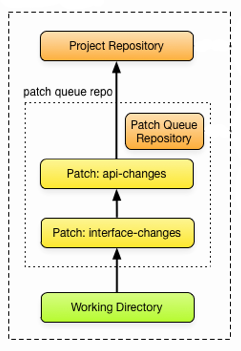
\includegraphics[width=1\textwidth]{mq-versioned.png}}
\end{column}
\end{columns}
\end{frame}

\begin{frame}
\transwipe[direction=90]
\frametitle{Работа с Mercurial Queues}
\centerline{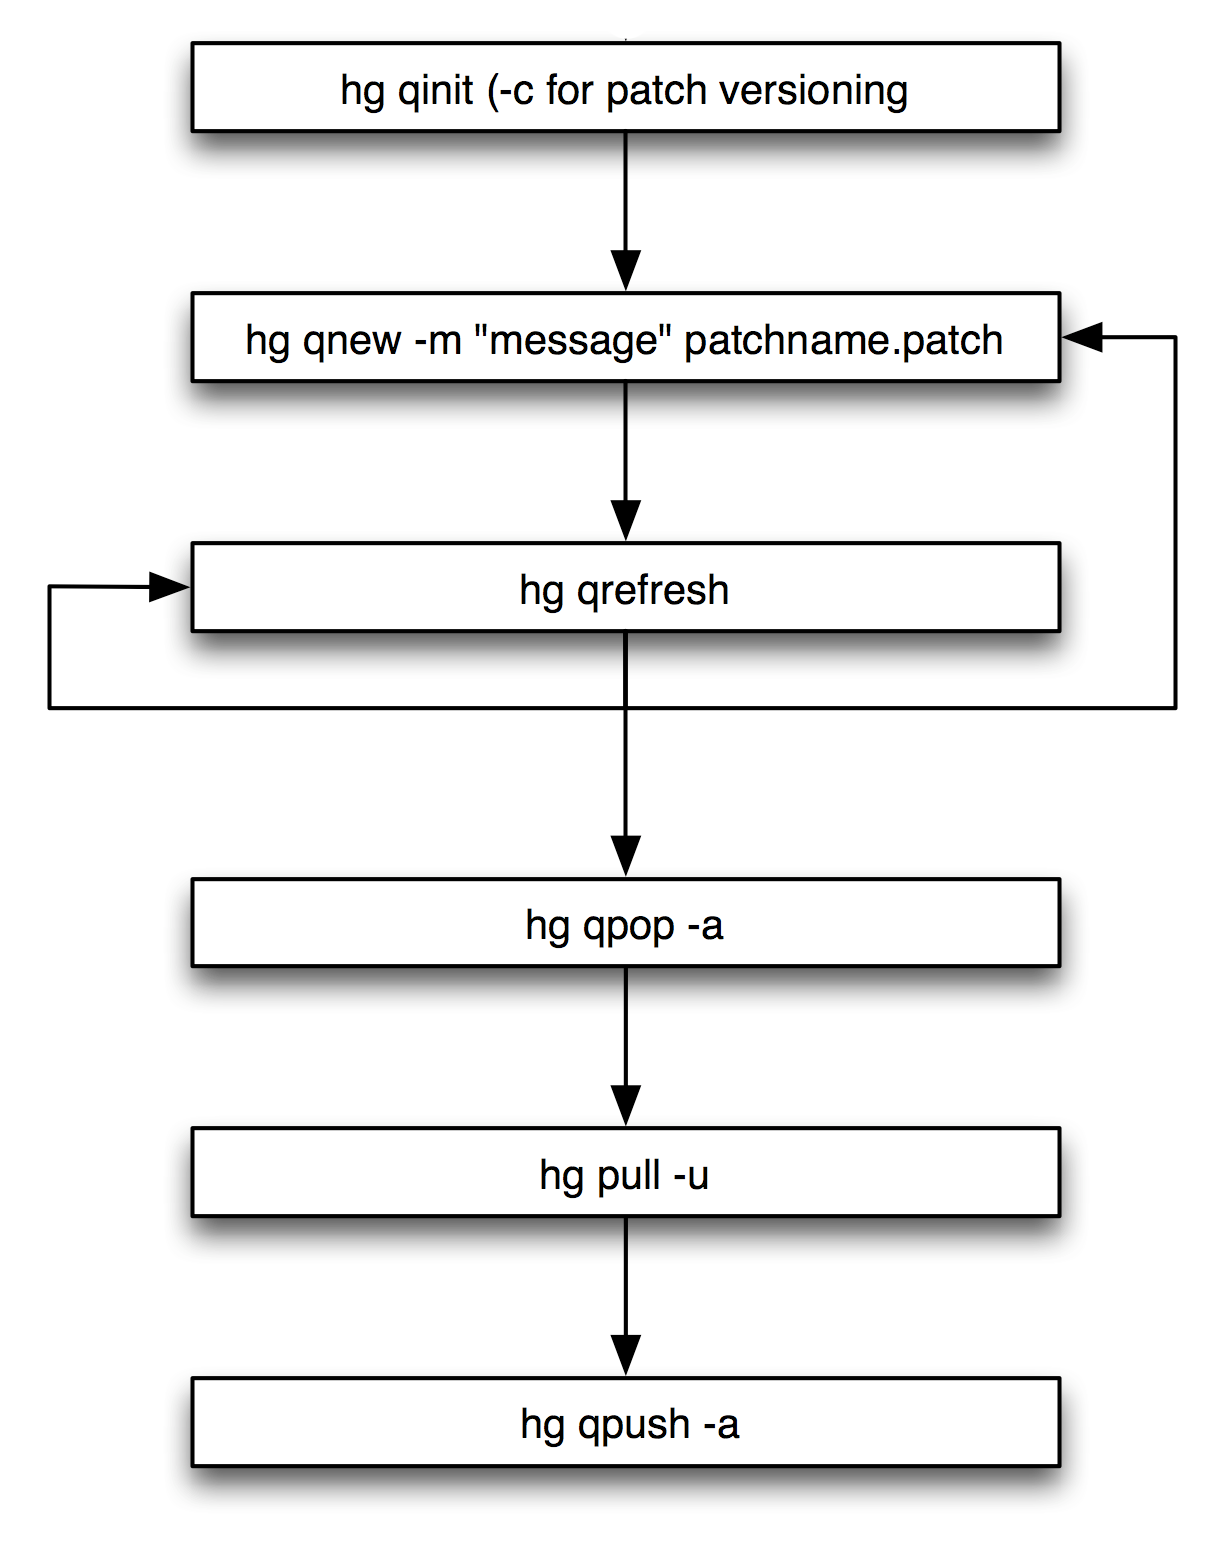
\includegraphics[width=0.5\textwidth]{mq-workflow.png}}
\end{frame}

\begin{frame}
\transwipe[direction=90]
\frametitle{Результаты}
\begin{block}{}
\begin{itemize}
  \item ?
  \item ?
  \item ?
  \item ?
  \item ?
\end{itemize}
\end{block}
\end{frame}


\begin{frame}
\transwipe[direction=90]
\frametitle{}
\centerline{\large{Cпасибо за внимание!}}
\hspace{2cm}
\centerline{\huge{Вопросы?}}
\end{frame}


\end{document}